\chapter{MIT bag model}

To model quark matter and the effect of these two properties,
physicists have come up with various \textbf{bag models}.
As illustrated in \cref{fig:lsm:confinement}, these models split the medium of the physical vacuum state into two phases.
The \emph{normal phase} is the background phase in which quarks are forbidden to exist -- remains of the non-confining medium that existed before the separation into two phases.
On top of the background, bubbles of \emph{hadron phase} are created inside which colorless combinations of quarks are confined.
Mathematically, the confinement is implemented by adding a bag constant $B$ to the grand potential density $\Omega$ of the quarks assumed to live inside the hadronic bubbles.
The bag constant is therefore defined as the energy difference between the hadronic phase and the normal phase,
and creating a hadronic bubble of volume $V$ costs the energy $B V$.
A positive bag constant gives a negative contribution to the pressure $P = -\Omega$,
hence confining the contents of the bag with an external pressure from the surrounding medium in the normal phase.

The \textbf{MIT bag model} is the simplest example.
Consider a star composed of up, down and strange quarks in the zero-temperature and massless approximation.
According to what we learned in \TODO{ref 4.12} and \eqref{eq:nstars:ur_eos}, the grand potential ``before bagging'' is
Pressure
\begin{equation}
	P(\mu) = \smashoperator{\sum_{f=\{u,d,s\}}} \frac{N_c \mu_f^4}{12 \pi^2}
	\qquad \text{and} \qquad
	\epsilon(\mu) = -P(\mu) + \smashoperator{\sum_{f=\{u,d,s\}}} \frac{N_c \mu_f^4}{3 \pi^2}.
\end{equation}
After ``bagging'' the quarks with a bag constant $B$,
\begin{equation}
\begin{split}
	P(\mu,B) = P(\mu) - B, \\
	\epsilon(\mu,B) = -P(\mu,B) + \smashoperator{\sum_{f=\{u,d,s\}}} \frac{N_c \mu_f^4}{3 \pi^2}.
	                = -P(\mu,B) + 4 (P(\mu,B) + B) = 4 P(\mu,B) + 4 B.
\end{split}
\end{equation}
The energy density and equation of state is then
\begin{equation}
	\epsilon(P) = -P + \sum_f \mu_f n_f = -P + \sum_f \frac{N_c \mu_f^4}{3 \pi^2} = -P + 4P = 3P
\end{equation}
To ``bag'' the quarks, the idea is 

In the early days of high density and temperature, the universe likely passed through a deconfined quark matter phase.
Today, matter is accreting by nuclear fusion in stars towards iron-56, seemingly representing the ground state of nuclear matter.
However, \cite{ref:strange_hypothesis_bodmer} and \cite{ref:strange_hypothesis_witten} has hypothesized that this state of matter is only \emph{metastable}.
Their \textbf{strange matter hypothesis} claims that the true ground state of nuclear matter is that of three-flavor matter consisting of up, down and strange quarks

\TODO{rewrite?}
We can use the presumed stability of two-flavor and three-flavor quark matter to determine a range of acceptable windows for the bag constant $B$.
Per baryon, iron-56 has an energy of $E/N_B = \epsilon/n_B = \SI{930}{\mega\electronvolt}$,
so if $\epsilon_2$ and $\epsilon_3$ are the energy densities of two-flavor and three-flavor quark matter,
we determine the bag constant $B$ such that
\TODO{at zero pressure?}
\begin{equation}
	\frac{\epsilon_3(0)}{n_B} < \SI{930}{\mega\electronvolt} < \frac{\epsilon_2(0)}{n_B} .
\label{eq:lsm:bag_stability}
\end{equation}
Only the two-flavor bound has been observed,
while the three-flavor bound is a quite reckless assumption that should certainly be taken with a grain of salt.
It will, however, be very useful to have \emph{some} bound for the bag constant in order to constrain the parameter space of equations of state later on.

% TODO: start here
\begin{figure}[bh!]
\centering
\tikzsetnextfilename{bag-mass-radius}
\begin{tikzpicture}
\begin{axis}[
	width=15cm, height=12cm,
	xlabel={$R \, / \, \si{\kilo\meter}$}, ylabel={$M \, / \, M_\odot$}, title={Mass-radius diagram for bag-model quark stars }, title style={yshift=2.0cm},
	xmin=0, xmax=15, ymin=0.0, ymax=2.2, xtick distance=1, ytick distance=0.1, minor tick num=9, grid=major,
	point meta=explicit, point meta min=32, point meta max=39,
	colorbar horizontal, colormap name=plasmarev, colorbar style={xlabel=$\log_{10} (P_c \, / \, \si{\pascal})$, xtick distance=1, minor x tick num=9, at={(0.5,1.03)}, anchor=south, xticklabel pos=upper},
	declare function={
		e0 = 4.266500881855304e+37;
	},
	legend pos=north east, legend cell align=right,
]
\tikzset{
	Bpin/.style={gray, sloped, allow upside down=true, rotate=180, yshift=+0.4cm, font=\small},
}
\addplot+ [mesh] table [x=R, y=M, meta expr={log10(\thisrow{P}*e0)}] {../code/data/MIT2F/stars_B14_144.dat}; % node [Bpin, pos=0.920] {$B = (\SI{27}{\mega\electronvolt})^4$};
\addplot+ [mesh] table [x=R, y=M, meta expr={log10(\thisrow{P}*e0)}] {../code/data/MIT2F/stars_B14_163.dat}; % node [Bpin, pos=0.920] {$B = (\SI{27}{\mega\electronvolt})^4$};
\end{axis}
\end{tikzpicture}
\caption{\TODO{MIT bag model 2 and 3 flavors}}
\end{figure}

\TODO{titles}

\TODO{units, $\hbar = c = G = k_B = 1$ or not?}

\TODO{organize project and master thesis together}

\TODO{color confinement, asymptotic freedom, bag models, etc.}
\begin{figure}
\centering
\tikzsetnextfilename{bag-model}
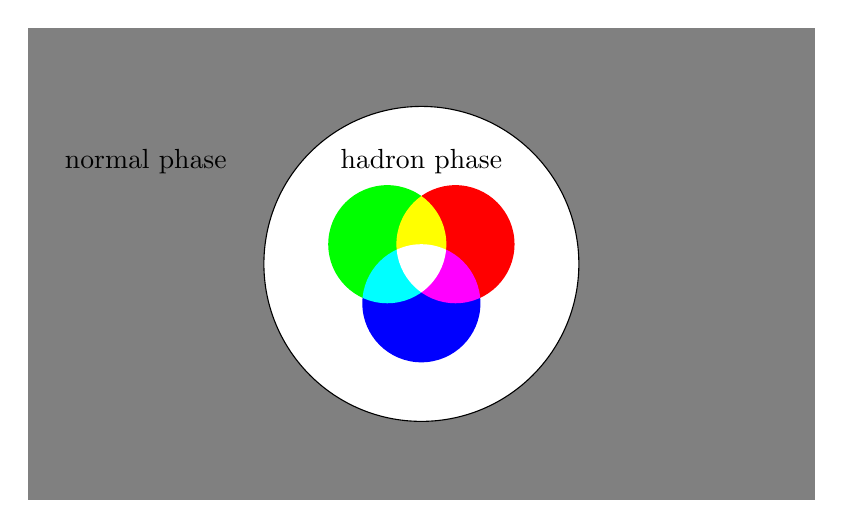
\begin{tikzpicture}
\fill [gray] (-5, -3) rectangle (+5, +3);

\draw [draw=black, fill=white] (0, 0) circle (2);
\begin{scope}[blend group=screen]
	\fill [fill=red]   (30:0.5)  circle (0.75) node {$u$};
	\fill [fill=green] (150:0.5) circle (0.75) node {$d$};
	\fill [fill=blue]  (270:0.5) circle (0.75) node {$s$};
\end{scope}
\node at (90:1.3) {hadron phase};
\node at (-3.5,1.3) {normal phase};
\end{tikzpicture}
\caption{\label{fig:master_intro:confinement}%
	\TODO{create different confinement vs deconfinement figure}
}
\end{figure}
